\documentclass[a4paper,notitlepage]{article}

\usepackage{polski}
\usepackage[utf8]{inputenc}
\usepackage[left=2cm,right=2cm,top=3cm,bottom=3cm]{geometry}
\usepackage{multirow}
\usepackage{graphicx}

\author{
	inż. Paweł Tobiszewski, 179769\\
	inż. Marcin Ważeliński, 179151
}
\title{
	\textbf{Face Comparator --- sprawozdanie}\\
	Systemy wspomagania decyzji - projekt\\
	czwartek, \hour{18}{55} -- \hour{20}{30}\\
	prowadzący: dr. inż. Dariusz Gąsior
}
\date{}

\newcommand{\hour}[2]{
	$#1^{\underline{#2}}$
}

\begin{document}
\maketitle

\section{Wstęp}
Podczas zajęć projektowych naszym zadaniem było zastosowanie metod poznanych na ćwiczeniach i w trakcie wykładu do zaimplementowania algorytmu wspomagającego rozwiązanie wybranego problemu decyzyjnego.
Wybranym przez nas problemem było wielokryterialne porównywanie twarzy, więc zastosowaliśmy metodę AHP.

\subsection{Przedstawienie problemu}
Aplikacja realizowana w trakcie projektu będzie pomagać rozwiązać problem wyboru najbardziej odpowiadającej użytkownikowi twarzy.
Kryteria pod względem których oceniane będą twarze poda sam użytkownik --- dla działania metody AHP ważna jest tylko ilość kryteriów, ich nazwy nie mają znaczenia dla działania algorytmu.

\section{Przykład zastosowania metody AHP do rozwiązania problemu wyboru twarzy}

Przykładowy problem wyboru twarzy:
\begin{itemize}
\item decyzje - 3 twarze: d1, d2, d3
\item kryteria - k1, k2, k3 (nazwy nie są ważne dla działania metody)
\end{itemize}

\begin{table}[!ht]
\centering
\caption{Macierz porównań kryteriów}
	\begin{tabular}{c|c|c|c}
		&	$K_1$	&	$K_2$	&	$K_3$\\ \hline
	$K_1$	&	$1.0$	&	$1.0$	&	$7.0$\\ \hline
	$K_2$	&	$1.0$	&	$1.0$	&	$3.0$\\ \hline
	$K_3$	&	$0.14$	&	$0.33$	&	$1.0$
	\end{tabular}
\end{table}
\begin{table}[!ht]
\centering
\caption{Macierz porównań decyzji względem pierwszego kryterium}
	\begin{tabular}{c|c|c|c}
		&	$D_1$	&	$D_2$	&	$D_3$\\ \hline
	$D_1$	&	$1.0$	&	$0.2$	&	$5.0$\\ \hline
	$D_2$	&	$5.0$	&	$1.0$	&	$7.0$\\ \hline
	$D_3$	&	$0.2$	&	$0.14$	&	$1.0$
	\end{tabular}
\end{table}
\begin{table}[!ht]
\centering
\caption{Macierz porównań decyzji względem drugiego kryterium}
	\begin{tabular}{c|c|c|c}
		&	$D_1$	&	$D_2$	&	$D_3$\\ \hline
	$D_1$	&	$1.0$	&	$3.0$	&	$9.0$\\ \hline
	$D_2$	&	$0.33$	&	$1.0$	&	$3.0$\\ \hline
	$D_3$	&	$0.11$	&	$0.33$	&	$1.0$
	\end{tabular}
\end{table}
\begin{table}[!ht]
\centering
\caption{Macierz porównań decyzji względem trzeciego kryterium}
	\begin{tabular}{c|c|c|c}
		&	$D_1$	&	$D_2$	&	$D_3$\\ \hline
	$D_1$	&	$1.0$	&	$0.2$	&	$0.11$\\ \hline
	$D_2$	&	$5.0$	&	$1.0$	&	$0.14$\\ \hline
	$D_3$	&	$9.0$	&	$7.0$	&	$1.0$
	\end{tabular}
\end{table}

\pagebreak
\subsection{Etap 1 --- wyznaczenie wektorów preferencji}
Metoda AHP polega na wyliczeniu rankingu decyzji, opierając się na tzw. wektorach preferencji --- obliczanych dla każdej z powyższych macierzy.
Aby wyznaczyć wektor preferencji, należy najpierw policzyć sumy w kolumnach macierzy. Następnie sumy te wykorzystane zostaną do znormalizowania macierzy.
Wektor preferencji wyznaczony jest poprzez uśrednienie wartości w wierszach znormalizowanych macierzy.

\begin{table}[!ht]
\centering
\caption{Wyznaczenie wektora preferencji dla macierzy porównań kryteriów}
	\begin{tabular}{ccccc}
		\begin{tabular}{c|c|c|c}
			&	$K_1$	&	$K_2$	&	$K_3$\\ \hline
		$K_1$	&	$1.0$	&	$1.0$	&	$7.0$\\ \hline
		$K_2$	&	$1.0$	&	$1.0$	&	$3.0$\\ \hline
		$K_3$	&	$0.14$	&	$0.33$	&	$1.0$\\
		\multicolumn{4}{c}{
			$c_1=
			\left[
				\begin{array}{ccc}
				2.14		&	2.33		&	11.0\\
				\end{array}
			\right]$
		}
		\end{tabular}
	&
	$\rightarrow$
	&
		\begin{tabular}{c|c|c|c}
			&	$D_1$	&	$K_2$	&	$K_3$\\ \hline
		$K_1$	&	$0.47$	&	$0.43$	&	$0.64$\\ \hline
		$K_2$	&	$0.47$	&	$0.43$	&	$0.27$\\ \hline
		$K_3$	&	$0.07$	&	$0.14$	&	$0.09$
		\end{tabular}
	&
	$\rightarrow$
	&
	$s_0=
	\left[
		\begin{array}{c}
		0.51\\
		0.39\\
		0.1\\
		\end{array}
		\right]$
	\end{tabular}
\end{table}
\begin{table}[!ht]
\centering
\caption{Wyznaczenie wektora sum dla macierzy porównań decyzji względem pierwszego kryterium}
	\begin{tabular}{ccccc}
		\begin{tabular}{c|c|c|c}
			&	$D_1$	&	$D_2$	&	$D_3$\\ \hline
		$D_1$	&	$1.0$	&	$0.2$	&	$5.0$\\ \hline
		$D_2$	&	$5.0$	&	$1.0$	&	$7.0$\\ \hline
		$D_3$	&	$0.2$	&	$0.14$	&	$1.0$\\
		\multicolumn{4}{c}{
			$c_1=
			\left[
				\begin{array}{ccc}
				6.20		&	1.34		&	13.0\\
				\end{array}
			\right]$
		}
		\end{tabular}
	&
	$\rightarrow$
	&
		\begin{tabular}{c|c|c|c}
			&	$D_1$	&	$D_2$	&	$D_3$\\ \hline
		$D_1$	&	$0.16$	&	$0.15$	&	$0.38$\\ \hline
		$D_2$	&	$0.81$	&	$0.74$	&	$0.54$\\ \hline
		$D_3$	&	$0.03$	&	$0.11$	&	$0.08$
		\end{tabular}
	&
	$\rightarrow$
	&
	$s_1=
	\left[
		\begin{array}{c}
		0.23\\
		0.70\\
		0.07\\
		\end{array}
	\right]$
	\end{tabular}
\end{table}
\begin{table}[!ht]
\centering
\caption{Wyznaczenie wektora preferencji dla macierzy porównań decyzji względem drugiego kryterium}
	\begin{tabular}{ccccc}
		\begin{tabular}{c|c|c|c}
			&	$D_1$	&	$D_2$	&	$D_3$\\ \hline
		$D_1$	&	$1.0$	&	$3.0$	&	$9.0$\\ \hline
		$D_2$	&	$0.33$	&	$1.0$	&	$3.0$\\ \hline
		$D_3$	&	$0.11$	&	$0.33$	&	$1.0$\\
		\multicolumn{4}{c}{
			$c_2=
			\left[
				\begin{array}{ccc}
				1.44		&	4.33		&	13.0\\
				\end{array}
			\right]$
		}
		\end{tabular}
	&
	$\rightarrow$
	&
		\begin{tabular}{c|c|c|c}
			&	$D_1$	&	$D_2$	&	$D_3$\\ \hline
		$D_1$	&	$0.69$	&	$0.69$	&	$0.69$\\ \hline
		$D_2$	&	$0.23$	&	$0.23$	&	$0.23$\\ \hline
		$D_3$	&	$0.08$	&	$0.08$	&	$0.08$
		\end{tabular}
	&
	$\rightarrow$
	&
	$s_2=
	\left[
		\begin{array}{c}
		0.69\\
		0.23\\
		0.08\\
		\end{array}
	\right]$
	\end{tabular}
\end{table}
\begin{table}[!ht]
\centering
\caption{Wyznaczenie wektora preferencji dla macierzy porównań decyzji względem trzeciego kryterium}
	\begin{tabular}{ccccc}
		\begin{tabular}{c|c|c|c}
			&	$D_1$	&	$D_2$	&	$D_3$\\ \hline
		$D_1$	&	$1.0$	&	$0.2$	&	$0.11$\\ \hline
		$D_2$	&	$5.0$	&	$1.0$	&	$0.14$\\ \hline
		$D_3$	&	$9.0$	&	$7.0$	&	$1.0$\\
		\multicolumn{4}{c}{
			$c_3=
			\left[
				\begin{array}{ccc}
				15.0		&	8.2		&	1.25\\
				\end{array}
			\right]$
		}
		\end{tabular}
	&
	$\rightarrow$
	&
		\begin{tabular}{c|c|c|c}
		$K_3$	&	$D_1$	&	$D_2$	&	$D_3$\\ \hline
		$D_1$	&	$0.07$	&	$0.02$	&	$0.09$\\ \hline
		$D_2$	&	$0.33$	&	$0.12$	&	$0.11$\\ \hline
		$D_3$	&	$0.6$	&	$0.85$	&	$0.8$
		\end{tabular}
	&
	$\rightarrow$
	&
	$s_3=
	\left[
		\begin{array}{c}
			0.06\\
			0.19\\
			0.75
		\end{array}
	\right]$
	\end{tabular}
\end{table}

\subsection{Wyznaczenie rankingu decyzji}
Ostateczny ranking decyzji jest złożeniem rankingów dla poszczególnych kryteriów z rankingiem samych kryteriów.
Aby wyliczyć ten ranking, należy wymnożyć macierz powstałą przez ,,sklejenie'' wektorów preferencji decyzji dla każdego z kryteriów przez wektor preferencji kryteriów.
\[ R = \left[ \begin{array}{ccc}	c_1	&	c_2	&	c_3 \end{array} \right] \times c_0 \]
\[
	R = \left[
		\begin{array}{ccc}
		c_{1}^{(1)}	&	c_{2}^{(1)}	&	c_{3}^{(1)}\\
		c_{1}^{(2)}	&	c_{2}^{(2)}	&	c_{3}^{(2)}\\
		c_{1}^{(3)}	&	c_{2}^{(3)}	&	c_{3}^{(3)}\\
		\end{array}
	\right]
	\times
	\left[
		\begin{array}{c}
		c_{0}^{(1)}\\
		c_{0}^{(2)}\\
		c_{0}^{(3)}\\
		\end{array}
	\right]
\]
\[
	R=
	\left[
	\begin{array}{ccc}
		0.23	&	0.69	&	0.06\\
		0.70	&	0.23	&	0.19\\
		0.07	&	0.08	&	0.75\\
	\end{array}
	\right]
	\times
	\left[
	\begin{array}{c}
		0.51\\
		0.39\\
		0.1\\
	\end{array}
	\right]
	=
	\left[
	\begin{array}{c}
		0.39\\
		0.46\\
		0.14\\
	\end{array}
	\right]
\]

\subsection{Test spójności}
\subsubsection{Definicja spójności}
Aby zapewnić poprawność wyniku, wszystkie macierze powinny być spójne, tzn. $\forall_{i,j,k} \left( a_{i,j} \cdot a_{j,k} = a_{i,k} \right)$.
Obliczanie tak zdefiniowanej spójności jest jednak kosztowne obliczeniowo, więc w praktyce stosuje się metody przybliżone.
Jedną z nich jest metoda Saaty'ego --- i ją właśnie wykorzystamy w naszej pracy.

Metoda ta opiera się na empirycznie wyliczonych współczynnikach, zależnych od rozmiaru macierzy. Dla macierzy $3 \times 3$ współczynnik $RI$ wynosi $0.58$.
Współczynnik spójności wyliczany za pomocą metody Saaty'ego wynosi
\[ CR = \frac{CI}{RI} \]
\[ CI = \frac{\lambda - n}{n - 1} \textrm{, gdzie $n$ --- rozmiar macierzy} \]
\[ \lambda = c \cdot s \textrm{, gdzie $c$ --- wektor sum, $s$ --- wektor preferencji} \]
Macierz jest spójna, jeżeli $CI < 0.1$

\subsubsection{Wyznaczenie spójności macierzy}
Macierz preferencji kryteriów
\[ \lambda_0 = \left[ \begin{array}{ccc} 2.14 & 2.33 & 11.0 \end{array} \right] \times \left[ \begin{array}{c} 0.51\\ 0.39\\ 0.1\\ \end{array} \right] = 3.1\]
\[ CI_0 = \frac{\lambda_0 - 3}{2} = \frac{3.1 - 3}{2} = 0.05 \]
\[ CR_0 = \frac{CI_0}{RI_3} = \frac{0.05}{0.58} = 0.09 < 0.1 \rightarrow \textrm{macierz spójna} \]

Macierz porównań decyzji względem pierwszego kryterium
\[ \lambda_1 = \left[ \begin{array}{ccc} 6.2 & 1.34 & 13.0 \end{array} \right] \times \left[ \begin{array}{c} 0.23\\ 0.70\\ 0.07\\ \end{array} \right] = 3.31 \]
\[ CI_1 = \frac{\lambda_1 - 3}{2} = \frac{3.31 - 3}{2} = 0.15 \]
\[ CR_1 = \frac{CI_1}{RI_3} = \frac{0.15}{0.58} = 0.26 > 0.1 \rightarrow \textrm{macierz niespójna} \]

Macierz porównań decyzji względem drugiego kryterium
\[ \lambda_2 = \left[ \begin{array}{ccc} 1.44 & 4.33 & 13.0 \end{array} \right] \times \left[ \begin{array}{c} 0.69\\ 0.23\\ 0.08\\ \end{array} \right] = 3.0 \]
\[ CI_2 = \frac{\lambda_2 - 3}{2} = \frac{3.0 - 3}{2}=0.0 \]
\[ CR_2 = \frac{CI_2}{RI_3} = \frac{0.0}{0.58} = 0.0 < 0.1 \rightarrow \textrm{macierz spójna} \]

Macierz porównań decyzji względem trzeciego kryterium
\[ \lambda_3 = \left[ \begin{array}{ccc} 15.0 & 8.2 & 1.25 \end{array} \right] \times \left[ \begin{array}{c} 0.06\\ 0.19\\ 0.75\\ \end{array} \right] = 3.4 \]
\[ CI_3 = \frac{\lambda_3 - 3}{2} =\frac{3.4 - 3}{2} = 0.2 \]
\[ CR_3 = \frac{CI_3}{RI_3} = \frac{0.2}{0.58} = 0.34 > 0.1 \rightarrow \textrm{macierz niespójna} \]

Niespójność macierzy nie implikuje niepoprawności otrzymanych wyników.
Metoda AHP zwróci wynik, nawet jeżeli część lub wszystkie macierze będą niespójne.
Jednak aby zapewnić poprawność wyniku, wszystkie macierze powinny spełniać kryterium spójności.
W rozważanym przykładzie 2 z macierzy okazały się być niespójne, więc otrzymane rezultaty nie mogą być w pełni wirygodne.

\section{Prezentacja aplikacji}
W wyniku pracy nad projektem powstala aplikacja umożliwiająca użytkownikowi dokonanie wyboru spośród kilku twarzy, porównując je pod względem określonych przez niego kryteriów.

Po włączeniu aplikacji ukazuje się ekran zawierający dwie listy (rys. \ref{img_start_screen}).
Po lewej stronie znajdują się twarze, jakie użytkownik dodał do porównania (domyślnie nie ma żadnych), po lewej natomiast nazwy kryteriów, pod względem których dokonywane będzie porównanie.
Na dole ekranu dostępne są przyciski pozwalające dodać/usunąć twarz lub kryterium oraz kontynuować działanie programu (przycisk stanie się aktywny po dodaniu co najmniej jedej twarzy oraz co najmniej jednego kryterium).
	\begin{figure}[!htp]
	\centering
	\caption{Startowy ekran aplikacji}
	\label{img_start_screen}
	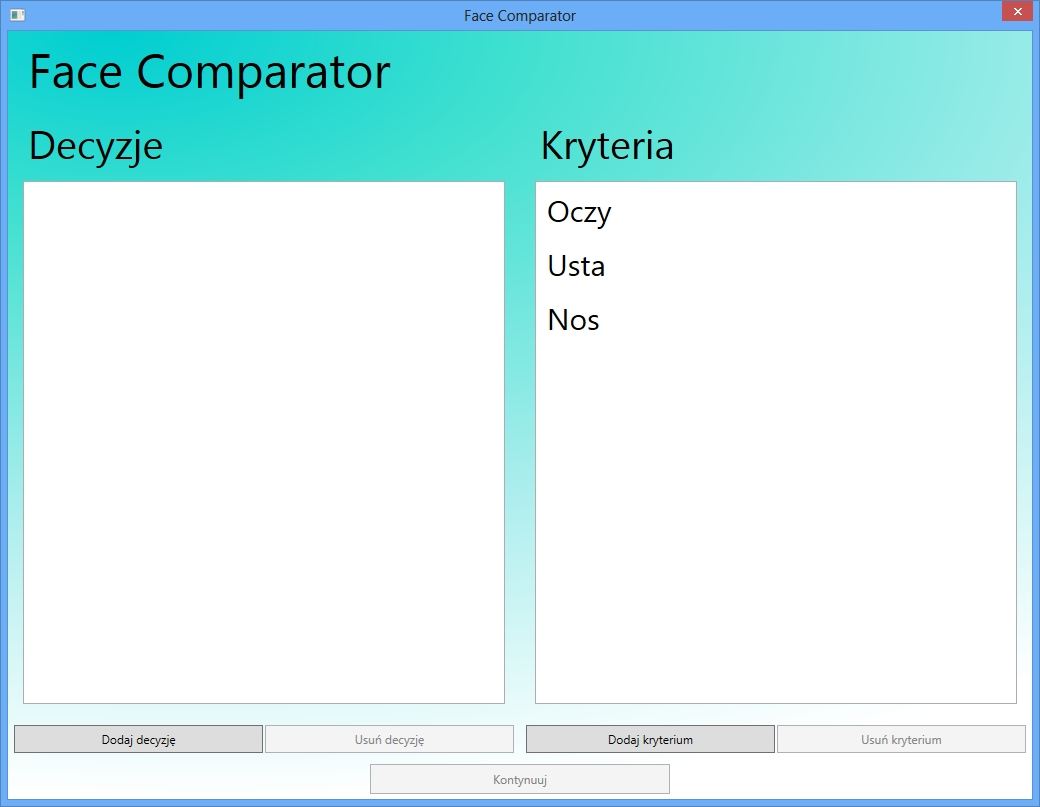
\includegraphics[width=0.8\textwidth]{img/startScreen}
	\end{figure}

Po wciśnięciu przycisku ,,dodaj kryterium'' zostaje otwarty dialog, w którym należy podać nazwę kryterium (rys. \ref{img_add_criterion_dialog}).
	\begin{figure}[!htp]
	\centering
	\caption{Dialog dodawania kryterium}
	\label{img_add_criterion_dialog}
	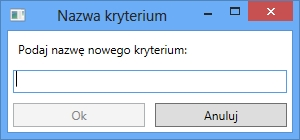
\includegraphics[scale=1.0]{img/addCriterionDialog}
	\end{figure}

Dodawanie twarzy polega na wybraniu zdjęcia, które będzie używane do porównań.
Dodane twarze pojawiają się na liście po lewej stronie (rys. \ref{img_faces_added}).
	\begin{figure}[!htp]
	\centering
	\caption{Ekran startowy po  dodaniu twarzy}
	\label{img_faces_added}
	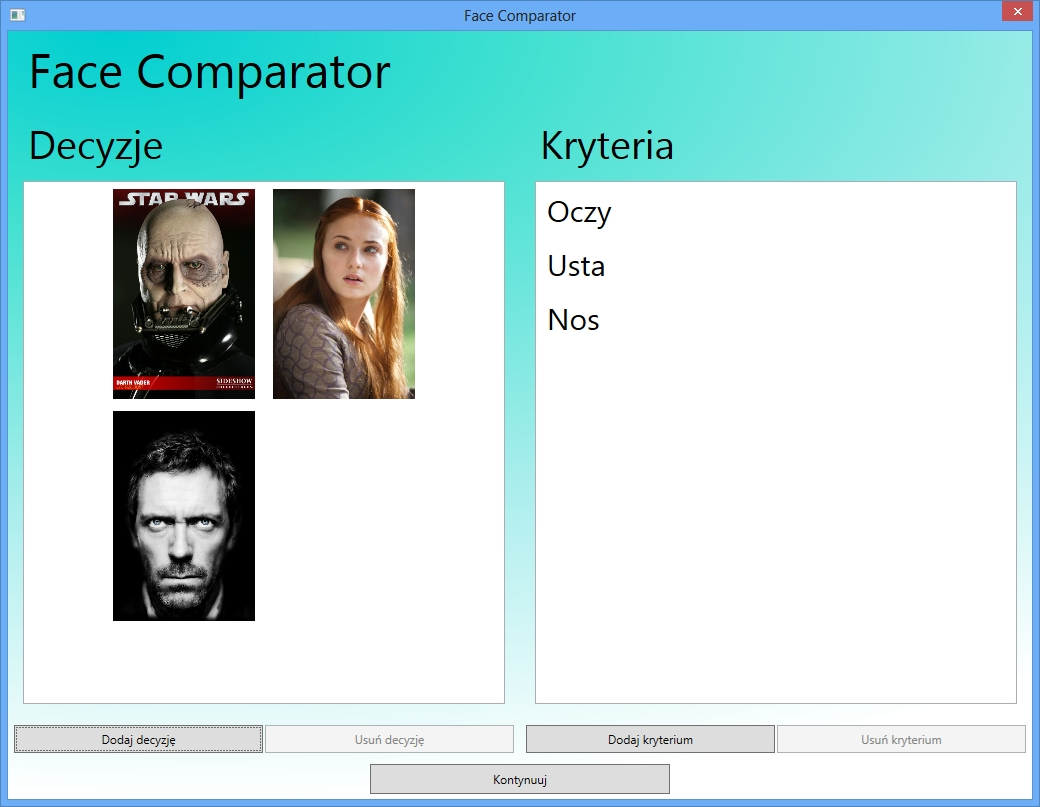
\includegraphics[width=0.8\textwidth]{img/facesAdded}
	\end{figure}

Kilknięcie przycisku ,,Kontynuuj'' przenosi użytkownika na kolejny ekran, gdzie dokonuje on porównania kryteriów (rys \ref{img_criterion_comparison}).
Przesuwając suwak w stronę odpowiedniego kryterium ustala on, które kryteria są dla niego ważniejsze.
Suwak na środku oznacza równe traktowanie kryteriów, natomiast maksymalne przesunięcie go w stronę wybranego kryterium oznacza ekstremalną preferencję tego kryterium nad znajdującym się po drugiej stronie.
	\begin{figure}[!htp]
	\centering
	\caption{Porównanie kryteriów}
	\label{img_criterion_comparison}
	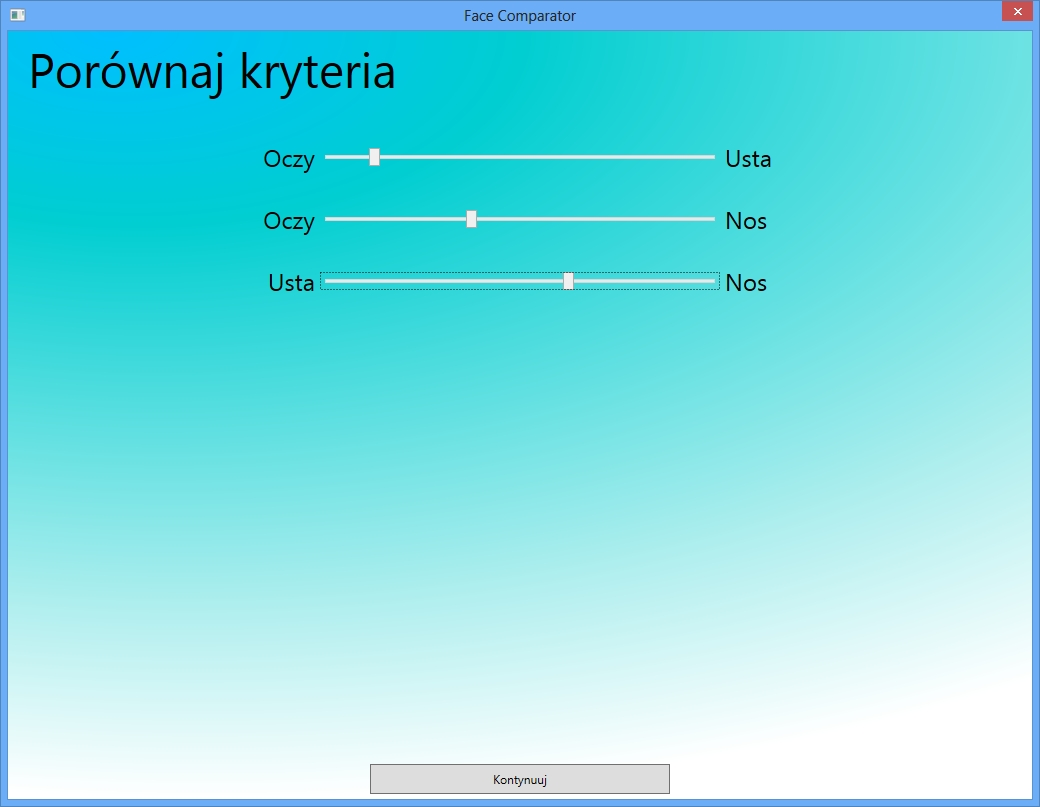
\includegraphics[width=0.8\textwidth]{img/criterionComparison}
	\end{figure}

Ponowne kliknięcie przycisku ,,Kontynuuj'' powoduje przejście do kolejnego ekranu, gdzie następuje porównanie twarzy względem pierwszego ze zdefiniowanych kryteriów (rys. \ref{img_decisions_comparison}).
Zasada działania suwaka jest taka sama, jak podczas porównywania kryteriów.
Jeżeli wykryta zostanie niespójność we wprowadzanych przez użytkownika danych, w prawym górnym rogu ekranu pojawi się stosowna informacja, widoczna na rysunku.
	\begin{figure}[!htp]
	\centering
	\caption{Porównanie twarzy}
	\label{img_decisions_comparison}
	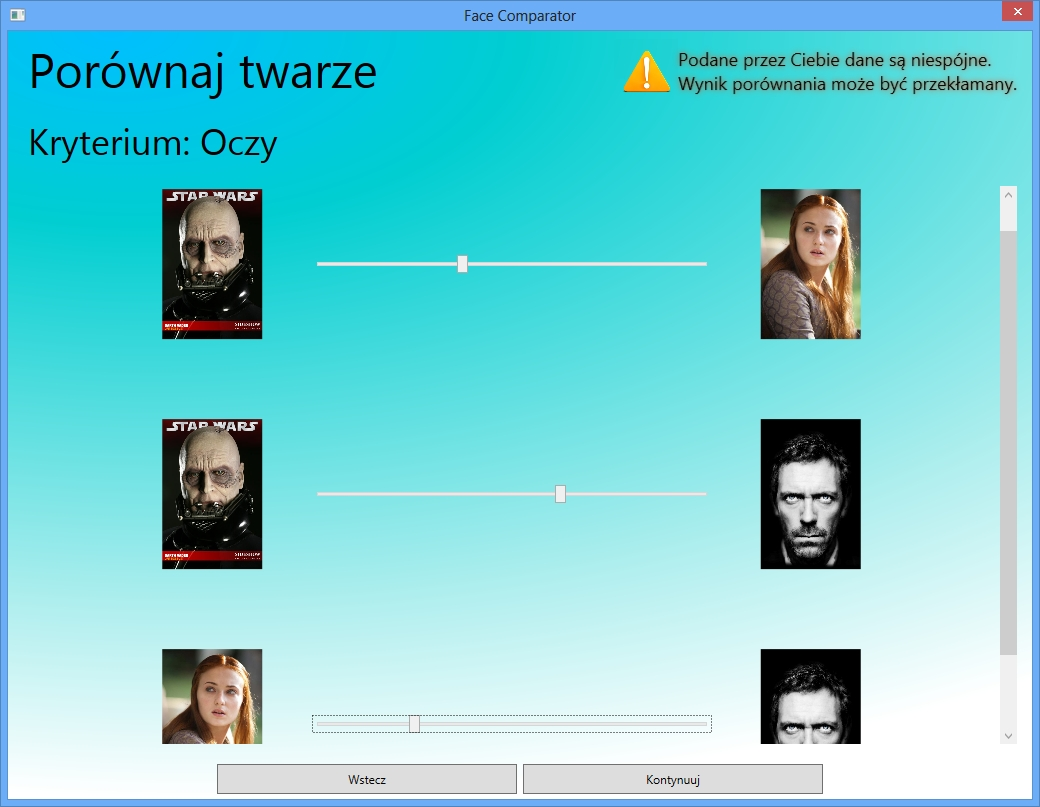
\includegraphics[width=0.8\textwidth]{img/decisionsComparison}
	\end{figure}

Aby powiększyć porównywane twarze, należy kliknąć na podświetlane pole pojawiające się w okolicach suwaka.
Pozwala to dokładniej przyjrzeć się twarzom i dokonać poprawnego porównania (rys. \ref{img_big_faces}).
	\begin{figure}[!htp]
	\centering
	\caption{Widok powiąkszonych twarzy}
	\label{img_big_faces}
	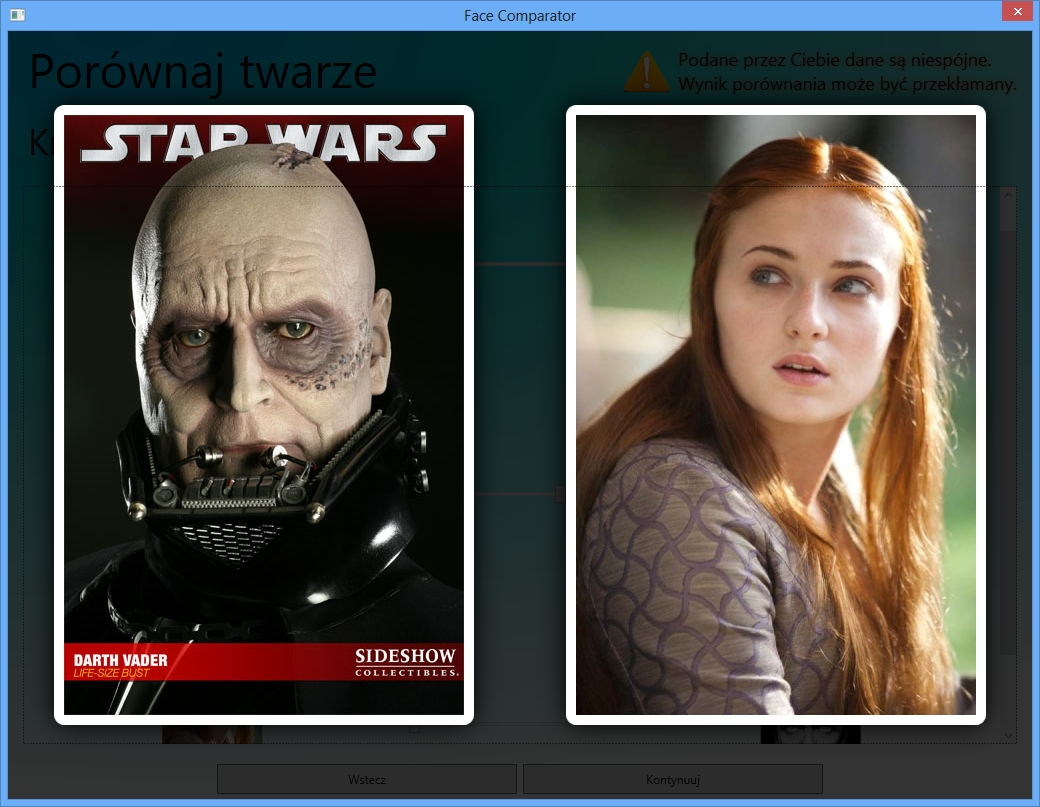
\includegraphics[width=0.8\textwidth]{img/bigFaces}
	\end{figure}

Następnie użytkownik dokonuje porównań twarzy względem pozostałych kryteriów.
Po zakończeniu porównań ukazuje się widok rankingu, obrazujący preferencje użytkownika (rys. \ref{img_ranking}).
	\begin{figure}[!htp]
	\centering
	\caption{Widok rankingu}
	\label{img_ranking}
	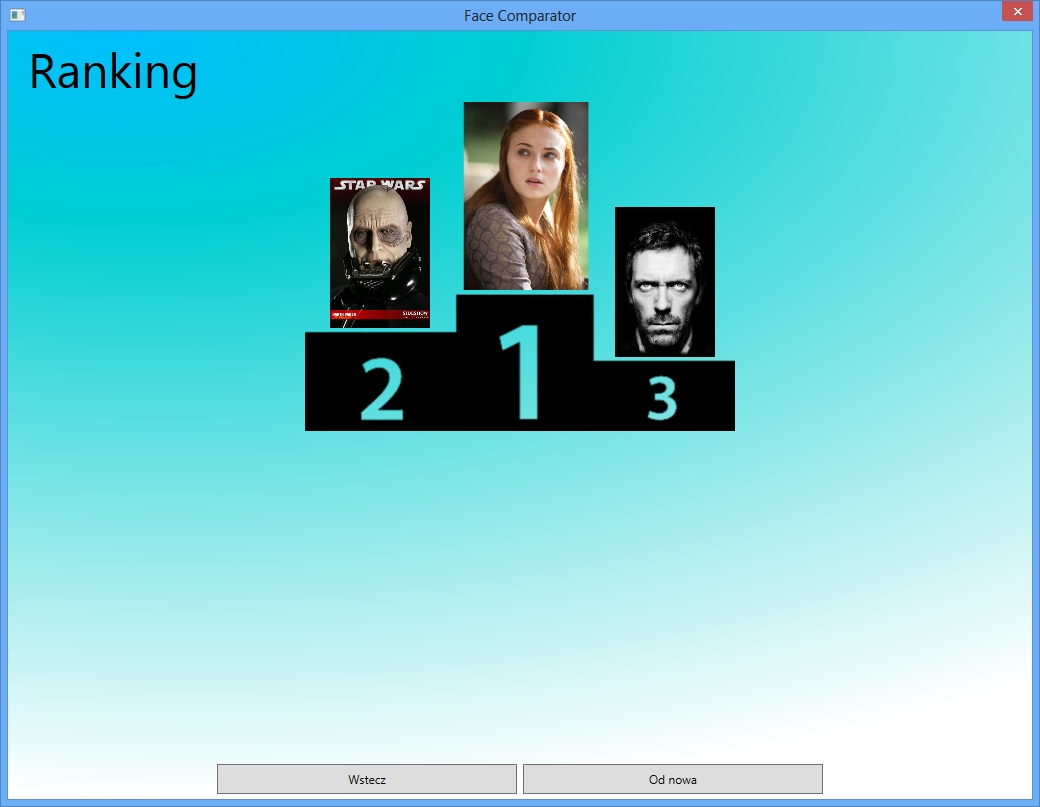
\includegraphics[width=0.8\textwidth]{img/ranking}
	\end{figure}
\end{document}
